% Assignment1 - Ajeesh T. Vijayan
\documentclass[11pt,a4paper]{article}
\usepackage[utf8]{inputenc}
\usepackage{array}
\usepackage{caption}
\usepackage{enumerate}
\usepackage{amsmath, amssymb}
\usepackage{array, makecell}
\usepackage{booktabs}
\usepackage{graphicx}
\usepackage[left=2.5cm,right=1.5cm,top=2cm,bottom=1.5cm]{geometry}
\usepackage{wrapfig}
\usepackage{float}
\usepackage{fancyhdr}
\usepackage{listings, lstautogobble}
\usepackage{listings-rust}
\usepackage{xcolor}

%New colors defined below
\definecolor{codegreen}{rgb}{0,0.6,0}
\definecolor{codegray}{rgb}{0.5,0.5,0.5}
\definecolor{codepurple}{rgb}{0.58,0,0.82}
\definecolor{backcolour}{rgb}{0.95,0.95,0.92}

%Code listing style named "mystyle"
\lstdefinestyle{mystyle}{
	backgroundcolor=\color{backcolour},   commentstyle=\color{codegreen},
	keywordstyle=\color{magenta},
	numberstyle=\tiny\color{codegray},
	stringstyle=\color{codepurple},
	basicstyle=\ttfamily\footnotesize,
	breakatwhitespace=false,         
	breaklines=true,                 
	captionpos=b,                    
	keepspaces=true,                 
	numbers=left,                    
	numbersep=3pt,                  
	showspaces=false,                
	showstringspaces=false,
	showtabs=false,                  
	tabsize=2
}

%"mystyle" code listing set
\lstset{style=mystyle}

\lstdefinestyle{DOS}
{
	backgroundcolor=\color{black},
	basicstyle=\scriptsize\color{white}\ttfamily
}

\pagestyle{fancy}
\lhead{Ajeesh T. Vijayan}
\rhead{Student No: 22077273}
\cfoot{\thepage}
\renewcommand{\headrulewidth}{0.4pt}
\renewcommand{\footrulewidth}{0.4pt}

\title{MA7010 – Number Theory for Cryptography - Assignment 1}
\author{Ajeesh Thattukunnel Vijayan}
\date{January 11\textsuperscript{th} 2024}

\newenvironment{numberlists}[1][3\parindent]
{\begin{list}{}{%
			\leftmargin=#1\relax
			\rightmargin=\leftmargin
			\itemsep=\jot
			\parsep=0pt
			\partopsep=0pt
			\labelsep=0pt}}
	{\end{list}}

\newcommand\numlist[2]{%
	\item[]\makebox[0pt][r]{$#1=\lbrack$}%
	\begingroup
	\begingroup\lccode`~=`,\lowercase{\endgroup\def~}{\mathcomma\penalty0 }%
	\mathcode`,="8000
	\thinmuskip=6mu plus 6mu minus 2mu
	$#2\rbrack$%
	\endgroup
}

\definecolor{dkgreen}{rgb}{0,0.6,0}
\definecolor{gray}{rgb}{0.5,0.5,0.5}
\definecolor{mauve}{rgb}{0.58,0,0.82}

\mathchardef\mathcomma=\mathcode`,
\newcommand{\roverline}[1]{\mathpalette\doroverline{#1}}
\newcommand{\doroverline}[2]{\overline{#1#2}}

\begin{document}
	
	\maketitle
	
	\begin{enumerate}[1.]
		\item Lower Range = 2800, Upper Range = 3100.
		\begin{enumerate}[(a)]
			\item List the elements of the set A = {all primes p in the range}, B = {all composite numbers in the range}.
		\end{enumerate}
		\begin{flushleft}
			\textbf{\textit{Answer:}}
			\begin{numberlists}
				\numlist{Primes}{2801, 2803, 2819, 2833, 2837, 2843, 2851, 2857, 2861, 2879, 2887, 2897, 2903, 2909, 2917, 2927, 2939, 2953, 2957, 2963, 2969, 2971, 2999, 3001, 3011, 3019, 3023, 3037, 3041, 3049, 3061, 3067, 3079, 3083, 3089}
				
				\numlist{Composites}{2800, 2802, 2804, 2805, 2806, 2807, 2808, 2809, 2810, 2811, 2812, 2813, 2814, 2815, 2816, 2817, 2818, 2820, 2821, 2822, 2823, 2824, 2825, 2826, 2827, 2828, 2829, 2830, 2831, 2832, 2834, 2835, 2836, 2838, 2839, 2840, 2841, 2842, 2844, 2845, 2846, 2847, 2848, 2849, 2850, 2852, 2853, 2854, 2855, 2856, 2858, 2859, 2860, 2862, 2863, 2864, 2865, 2866, 2867, 2868, 2869, 2870, 2871, 2872, 2873, 2874, 2875, 2876, 2877, 2878, 2880, 2881, 2882, 2883, 2884, 2885, 2886, 2888, 2889, 2890, 2891, 2892, 2893, 2894, 2895, 2896, 2898, 2899, 2900, 2901, 2902, 2904, 2905, 2906, 2907, 2908, 2910, 2911, 2912, 2913, 2914, 2915, 2916, 2918, 2919, 2920, 2921, 2922, 2923, 2924, 2925, 2926, 2928, 2929, 2930, 2931, 2932, 2933, 2934, 2935, 2936, 2937, 2938, 2940, 2941, 2942, 2943, 2944, 2945, 2946, 2947, 2948, 2949, 2950, 2951, 2952, 2954, 2955, 2956, 2958, 2959, 2960, 2961, 2962, 2964, 2965, 2966, 2967, 2968, 2970, 2972, 2973, 2974, 2975, 2976, 2977, 2978, 2979, 2980, 2981, 2982, 2983, 2984, 2985, 2986, 2987, 2988, 2989, 2990, 2991, 2992, 2993, 2994, 2995, 2996, 2997, 2998, 3000, 3002, 3003, 3004, 3005, 3006, 3007, 3008, 3009, 3010, 3012, 3013, 3014, 3015, 3016, 3017, 3018, 3020, 3021, 3022, 3024, 3025, 3026, 3027, 3028, 3029, 3030, 3031, 3032, 3033, 3034, 3035, 3036, 3038, 3039, 3040, 3042, 3043, 3044, 3045, 3046, 3047, 3048, 3050, 3051, 3052, 3053, 3054, 3055, 3056, 3057, 3058, 3059, 3060, 3062, 3063, 3064, 3065, 3066, 3068, 3069, 3070, 3071, 3072, 3073, 3074, 3075, 3076, 3077, 3078, 3080, 3081, 3082, 3084, 3085, 3086, 3087, 3088, 3090, 3091, 3092, 3093, 3094, 3095, 3096, 3097, 3098, 3099, 3100}
			\end{numberlists}

			The below images depicts the execution of the code on a powershell terminal:

			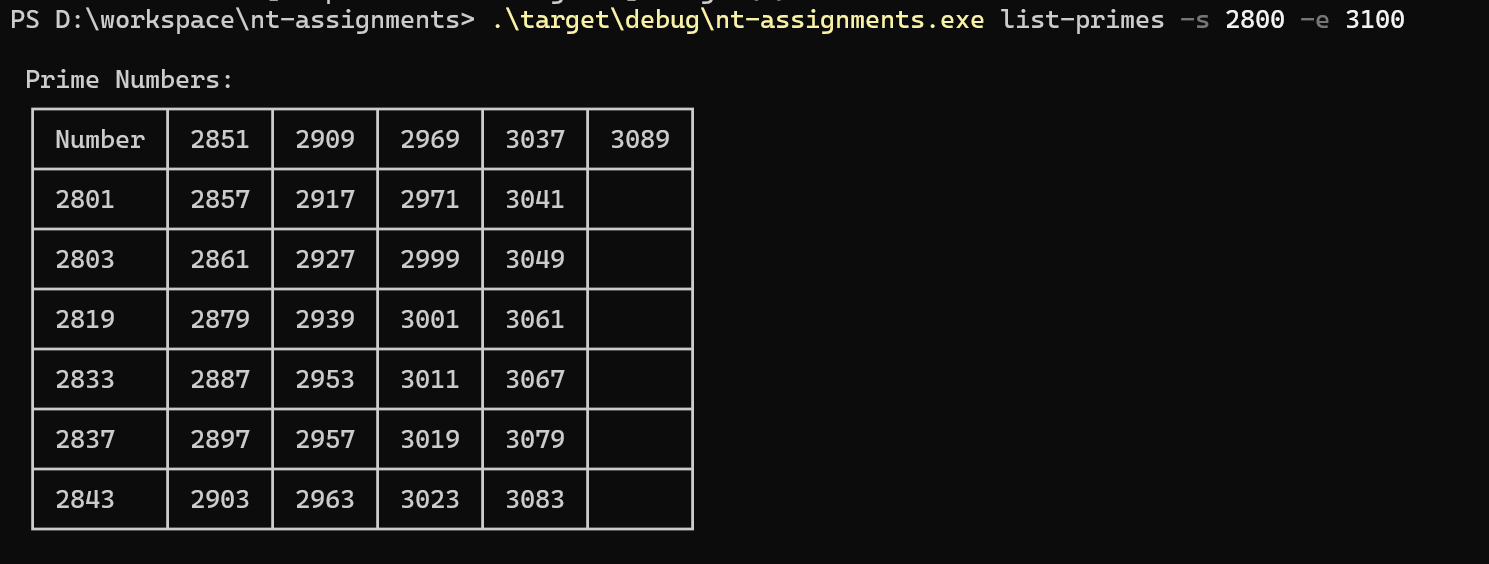
\includegraphics[width=\textwidth]{primes.png}
			\label{figure1:primes}
			
			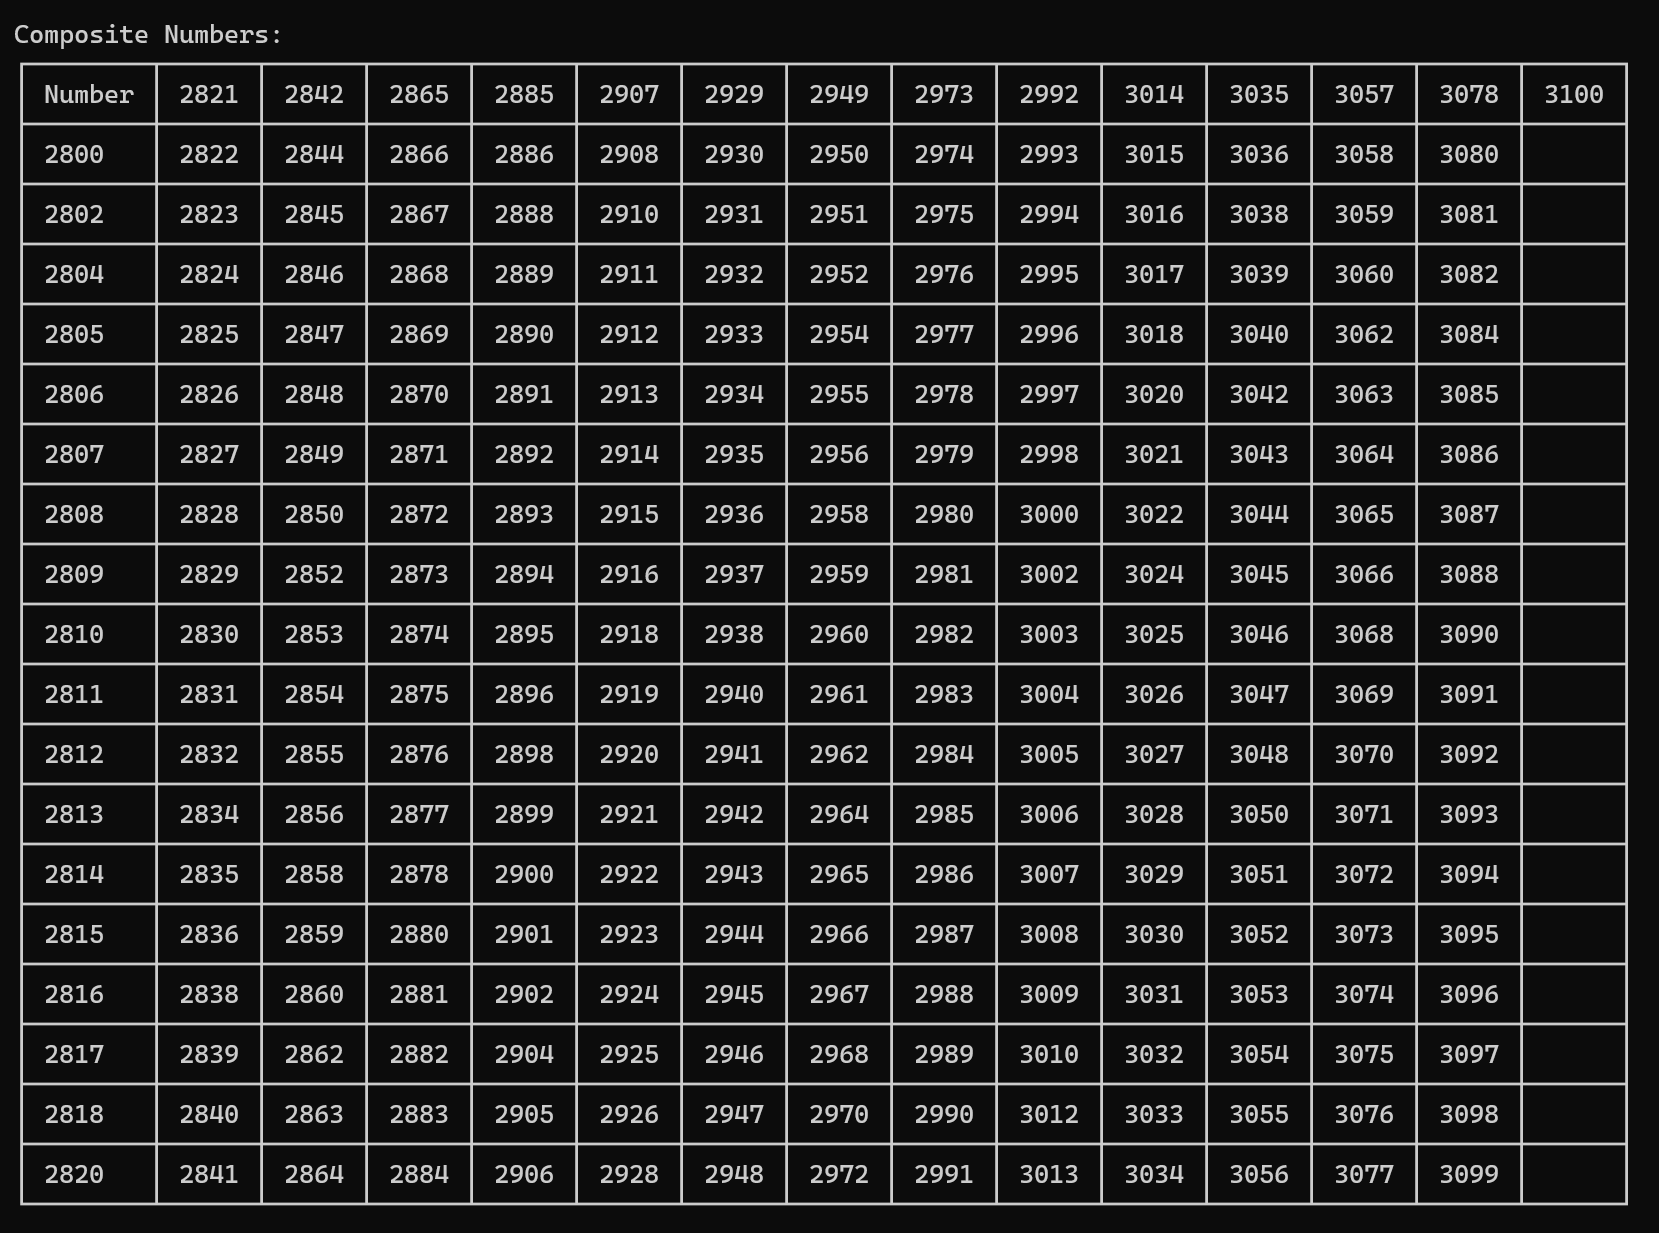
\includegraphics[width=\textwidth]{composites.png}
			\label{figure2:composites}

			\begin{lstlisting}[language=Rust, basicstyle=\tiny, caption=Prime Number Sieve]

			/// Returns a boolean representing if the given number is prime or not
			///
			/// # Arguments
			///
			/// * `n` - A BigInt
			///
			/// # Examples
			///
			/// ```
			/// use crate::primality::is_prime_trial_division_parallel;
			/// let is_prime = is_prime_trial_division_parallel(BigInt::from(100u64));
			/// ```
			pub fn is_prime_trial_division_parallel(n: &BigInt) -> bool {
				let (zero, one, _two) = (BigInt::from(0u64), BigInt::from(1u64), BigInt::from(2u64));
				let three = BigInt::from(3u64);
				
				// returns true if the number is 2 or 3
				if n <= &three {
					return n > &one;
				}
				
				if n % 2 == zero || n % 3 == zero {
					return false;
				}
				
				let upper_bound = n.sqrt() + 1; // +1 to get the ceiling value
				
				if let Some(_divisor) = range_inclusive(BigInt::from(5u64), upper_bound)
				.par_bridge()
				.into_par_iter()
				.find_first(|divisor| n % divisor == zero)
				{
					false
				} else {
					true
				}
			}

			\end{lstlisting}

			The above code verifies the primality of a number using trial division. It a sequence of numbers from $2$ to $sqrt(n) + 1$ and divides these numbers into chunks of blocks and checks the divisibility in parallel to speed up the execution.
			
			\bigbreak
			The below command execute the Prime Number Sieve:
			\begin{lstlisting}[style=DOS, caption=Example command - Prime Number Sieve]

				D:\workspace\nt-assignments>.\nt-assignments.exe list-primes -s 2800 -e 3100
			\end{lstlisting}
		\end{flushleft}
		
		\begin{enumerate}[(b)]
			\item List the elements of the set C where C = \{composite numbers n = pq in your range which are the product of exactly two distinct primes p and q\}.
		\end{enumerate}
		\begin{flushleft}
			\textbf{\textit{Answer:}} $H = \langle a \rangle = \{e, (1234), (13)(24), (1432)\}$
			
			If Hg is the right coset containing g, then we use $\bar{g}$ to represent Hg; hence: \smallskip \\
			
			coset containing $a$: $\displaystyle\overline{a} = \{(1234),(13)(24),(1432),e\}$ \\
			coset containing $b$: $\displaystyle\overline{b} = \{(13)(5678),(14)(23)(5678),(24)(5678),(12)(34)(5678)\}$ \\
			coset containing $b^2$: $\displaystyle\overline{b^2} = \{(57)(68),(1234)(57)(68),(13)(24)(57)(68),(1432)(57)(68)\}$ \\
			coset containing $b^3$: $\displaystyle\overline{b^3} = \{(13)(5876),(14)(23)(5876),(24)(5876),(12)(34)(5876)\}$ \\
			
			\begin{multline*}
				G/\langle a \rangle = \{\displaystyle\overline{a}, \displaystyle\overline{b}, \displaystyle\overline{b^2}, \displaystyle\overline{b^3}\} \\
			\end{multline*}
			
			This quotient group $G/\langle a \rangle $ is cyclic as we can generate the the whole group using the element $\displaystyle\overline{b}$
			
			By Lagrange's theorem, the order of a group is given by $|G| = |G/H|\times[G:H] = 4\times4 = 16$
		\end{flushleft}
		
		\begin{enumerate}[(c)]
			\item Show that $Z(G) = \langle a^2, b^2 \rangle$.
		\end{enumerate}
		\begin{flushleft}
			\textbf{\textit{Answer:}} The center of a group commutes with all other elements in the group. i.e., $Z(G) = \{g \in G | gs = sg  \forall s \in G\}$\\
			
			Given $Z(G) =  \langle a^2, b^2 \rangle = \{e, a^2, b^2, a^2b^2\} = \{e, (13)(24), (57)(68), (13)(24)(57)(68)\}$
			
			\begin{table}[H]
				\resizebox{\textwidth}{!}{\begin{tabular}{|r|r|r|r|r|r|r|r|c}
						\hline
						$\circ$ & $G = \{e, (13)(24), (57)(68), (13)(24)(57)(68)\}$\\
						\hline
						e & $eG = Ge$ \\
						\hline
						$a = (1234)$ & \begin{tabular}{c@{}}$aG = \{(1234), (1432), (1234)(57)(68), (1432)(57)(68)\}$ \\ $Ga = \{(1234), (1432), (1234)(57)(68), (1432)(57)(68)\}$\end{tabular} \\
						\hline
						$a^2 = (13)(24)$ & \begin{tabular}{@{}c@{}}$a^2G = \{(13)(24), e, (13)(24)(57)(68), (57)(68)\}$ \\ $Ga^2 = \{(13)(24), e, (13)(24)(57)(68), (57)(68) \}$\end{tabular} \\
						\hline
						$a^3 = (1432)$ & \begin{tabular}{@{}c@{}}$a^3G = \{(1432), (1234), (1432)(57)(68), (1234)(57)(68)\}$ \\ $Ga^3 = \{(1432), (1234), (1432)(57)(68), (1234)(57)(68)\}$\end{tabular} \\
						\hline
						$b = (13)(5678)$ & \begin{tabular}{@{}c@{}}$bG = \{(13)(5678), (24)(5876), (24)(5876)\}$ \\ $Gb = \{(13)(5678), (24)(5876), (24)(5876)\}$\end{tabular} \\
						\hline
						$b^2 = (57)(68)$ & \begin{tabular}{@{}c@{}}$b^2G = \{(57)(68), (13)(24)(57)(68), (13)(24)\}$ \\ $Gb^2 = \{(57)(68), (13)(24)(57)(68),(13)(24)\}$\end{tabular} \\
						\hline
						$b^3 = (13)(5876)$ & \begin{tabular}{@{}c@{}}$b^3G = \{(13)(5876), (24)(5876),(13)(5678),(24)(5678) \}$ \\ $Gb^3 = \{(13)(5876), (24)(5876), (13)(5678), (24)(5678)\}$\end{tabular} \\
						\hline
						$ab = (14)(23)(5678)$ & \begin{tabular}{@{}c@{}}$abG = \{(14)(23)(5678), (12)(34)(5678), (14)(23)(5876), (12)(34)(5876)\}$ \\ $Gab = \{(14)(23)(5678), (12)(34)(5678), (14)(23)(5876), (12)(34)(5876)\}$\end{tabular} \\
						\hline
						$ab^2 = (1234)(57)(68)$ & \begin{tabular}{@{}c@{}}$ab^2G = \{(1234)(57)(68), (1432)(57)(68), (1234), (1432)\}$ \\ $Gab^2 = \{(1234)(57)(68), (1432)(57)(68), (1234), (1432)\}$\end{tabular}\\
						\hline
						$ab^3 = (14)(23)(5876)$ & \begin{tabular}{@{}c@{}}$ab^3G = \{(14)(23)(5876), (12)(34)(5876), (14)(23)(5678), (12)(34)(5678)\}$ \\ $Gab^3 = \{(14)(23)(5876), (12)(34)(5876), (14)(23)(5678), (12)(34)(5678)\}$\end{tabular}\\
						\hline
						$ba^2 = (24)(5678)$ & \begin{tabular}{@{}c@{}}$ba^2G = \{(24)(5678), (13)(5678), (24)(5876), (13)(5876)\}$ \\ $Gba^2 = \{(24)(5678), (13)(5678), (24)(5876), (13)(5876)\}$\end{tabular} \\
						\hline
						$b^2a^2 = (13)(24)(57)(68)$ & \begin{tabular}{@{}c@{}}$b^2a^2G = \{(13)(24)(57)(68), (57)(68), (13)(24), e\}$ \\ $b^2a^2G = \{(13)(24)(57)(68), (57)(68), (13)(24), e\}$\end{tabular} \\
						\hline
						$a^2b^3 = (24)(5876)$ & \begin{tabular}{@{}c@{}}$a^2b^3G = \{(24)(5876), (13)(5876), (24)(5678), (13)(5678)\}$ \\ $Ga^2b^3 = \{(24)(5876), (13)(5876), (24)(5678), (13)(5678)\}$\end{tabular} \\
						\hline
						$ba = (12)(34)(5678)$ & \begin{tabular}{@{}c@{}}$baG = \{(12)(34)(5678), (14)(23)(5678), (12)(34)(5876), (14)(23)(5876)\}$ \\ $Gba = \{(12)(34)(5678), (14)(23)(5678), (12)(34)(5876), (14)(23)(5876)\}$\end{tabular} \\ 
						\hline
						$b^2a^3 = (1432)(57)(68)$ & \begin{tabular}{@{}c@{}}$b^2a^3G = \{(1432)(57)(68), (1234)(57)(68), (1432), (1234)\}$ \\ $Gb^2a^3 = \{(1432)(57)(68), (1234)(57)(68), (1432), (1234)\}$\end{tabular} \\
						\hline
						$b^3a = (12)(34)(5876)$ & \begin{tabular}{@{}c@{}}$b^3aG = \{(12)(34)(5876), (14)(23)(5876), (12)(34)(5678), (14)(23)(5678)\}$ \\ $Gb^3a = \{(12)(34)(5876), (14)(23)(5876), (12)(34)(5678), (14)(23)(5678)\}$\end{tabular} \\
						\hline
				\end{tabular}}
			\end{table}  
			
			From the table above, it's evident that all elements of G commute with $Z(G) = \langle a^2, b^2 \rangle$ and hence Z(G) is the center of the group.          
		\end{flushleft}
		\begin{enumerate}[(d)]
			\item Find the conjugacy classes of G expressing their elements as permutations
		\end{enumerate}
		\begin{flushleft}
			\textbf{\textit{Answer:}} 
			\begin{multline*}
				G = \{e, (1234), (13)(24), (1432), (13)(5678), (57)(68), (13)(5876), (14)(23)(5678), \\
				(1234)(57)(68), (14)(23)(5876), (24)(5678), (13)(24)(57)(68), (24)(5876), \\
				(12)(34)(5678), (1432)(57)(68), (12)(34)(5876)\}
			\end{multline*}
			
			$g = (1234)$
			\begin{table}[H]
				\begin{tabular}{|r|r|r|r|r|r|r|r|}
					\hline
					$\sigma(1234)\sigma^{-1}$ & (1234) & (1432) \\
					\hline
				\end{tabular}
			\end{table}
			
			$g = (13)(5678)$
			\begin{table}[H]
				\begin{tabular}{|r|r|r|r|r|r|r|r|}
					\hline
					$\sigma(13)(5678)\sigma^{-1}$ & (13)(5678) & (24)(5678) \\
					\hline
				\end{tabular}
			\end{table}
			
			$g = (13)(5876)$
			\begin{table}[H]
				\begin{tabular}{|r|r|r|r|r|r|r|r|}
					\hline
					$\sigma(13)(5876)\sigma^{-1}$ & (13)(5876) & (24)(5876) \\
					\hline
				\end{tabular}
			\end{table}
			
			$g = (14)(23)(5678)$
			\begin{table}[H]
				\begin{tabular}{|r|r|r|r|r|r|r|r|}
					\hline
					$\sigma(14)(23)(5678)\sigma^{-1}$ & (14)(23)(5678) & (12)(34)(5678) \\
					\hline
				\end{tabular}
			\end{table}
			
			$g = (1234)(57)(68)$
			\begin{table}[H]
				\begin{tabular}{|r|r|r|r|r|r|r|r|}
					\hline
					$\sigma(1234)(57)(68)\sigma^{-1}$ & (1234)(57)(68) & (1432)(57)(68) \\
					\hline
				\end{tabular}
			\end{table}
			
			$g = (14)(23)(5876)$
			\begin{table}[H]
				\begin{tabular}{|r|r|r|r|r|r|r|r|}
					\hline
					$\sigma(14)(23)(5876)\sigma^{-1}$ & (14)(23)(5876) & (12)(34)(5876) \\
					\hline
				\end{tabular}
			\end{table}
			
			Trivial Conjugacy Classes
			\begin{table}[H]
				\begin{tabular}{|r|r|r|r|r|r|r|r|}
					\hline
					e & (13)(24) & (57)(68) & (13)(24)(57)(68) \\
					\hline
				\end{tabular}
			\end{table}   
		\end{flushleft}
	\end{enumerate}
	
	\begin{enumerate}[3.]
		\item Let G be a group such that $126 \le |G| \le 132$. Given that G is simple find the possible values for $|G|$. In each case, justify your answer.
	\end{enumerate}
	
	\begin{flushleft}
		\textbf{\textit{Answer:}}
		A group G is simple if the only normal subgroups are the trivial subgroup $\{e\}$ and the improper subgroup G itself.\\
		\medskip
		Given $\mathbf{126 \le |G| \le 132}$. Let's go through each numbers
		\begin{enumerate}[(a)]
			\item $\mathbf{|G| = 126}$.
			Upon prime factorization $|G| = 2\times3^2\times7$. Let $n_7$ represents the number of Sylow 7-subgroups in G. By Sylow's third theorem,\medskip \\             
			$n_7 \equiv 1(\textrm{mod}\ 7)$ and $n_7|18$\smallskip\\
			Hence $n_7 = 1$ means that there exists a unique Sylow 7-subgroup of order 7 and it is normal. So $|G|=126$ is not a valid order for a simple group.
			
			\item $\mathbf{|G| = 127}$.\\
			127 is a prime number. By Lagrange's theorem, the order of a subgroup must divide the order of the group. The only divisors of 127 are 1 and 127 itself and hence there are no proper normal subgroups for a group or order 127. So the group is \textbf{Simple.}
			
			\item $\mathbf{|G| = 128}$. \\
			The prime factorization is given by $128 = 2^7$. It's a p-group and hence the center of the group Z(G) is not trivial. Also Z(G) is a proper normal subgroup of G. By Cauchy's theorem, if $|G| = n$ and if $n = pm$ where p is a prime and $p|m$, then $\exists g \in G$ such that $g^p = e \implies |g| = p$\medskip\\
			
			In  our case, we can write $|G|$ as $128 = 2\times2^6$. So $p = 2$ and $m = 2^6$. This implies that we can generate the entire group using the single element 'g', i.e, 
			
			$G = \langle g | g^{128}=e\rangle$ and this is cyclic. Every cyclic group is abelian and hence Z(G) = G, but the order is not prime and hence \textbf{not simple}
			
			\item $\mathbf{|G| = 129}$. Upon prime factorization, $129 = 3\times43$\\. 
			
			By Lagrange's theorem, the order of a subgroup must divide the order of the group. The factors of 129 are $\{1, 3, 43, 129\}$. For a simple group, the only normal subgroups are the trivial group $\{e\}$ and the improper subgroup G itself. So subgroups of order 1 and 129 are out of question here. We need to verify if subgroups of order 3 and 43 are normal.\medskip\\
			
			Let's verify if we have a Sylow 43-subgroup in G. By Sylow's third theorem, $n_{43} \equiv 1(\textrm{mod}\ 43)$ and $n_{43}|3$.\\
			We have $n_{43} = 1$ satisfies the condition. That means there exists a unique proper normal Sylow 43-subgroup for a group of order 129. So the group is \textbf{not simple.}
			
			\item $\mathbf{|G| = 130}$.\medskip\\
			
			$|G| = 2\times5\times13$. If we consider Sylow 13-subgroup in G, by Sylow's third theorem, $n_{13} \equiv 1(\textrm{mod}\ 13)$ and $n_{13}|10$.\\
			Only $n_{13} = 1$ can satisfies these two conditions. That means there exists a unique proper normal Sylow 13-subgroup for a group of order 130. So the group is \textbf{not simple.}
			
			\item $\mathbf{|G| = 131}$.\\
			131 is a prime number. By Lagrange's theorem, the order of a subgroup must divide the order of the group. The only factors of 131 are 1 and 131 itself and hence there are no proper normal subgroups for a group or order 131. So the group is \textbf{Simple.}
			
			\item $\mathbf{|G| = 132}$.\\
			
			The prime factorization of $|G|$ is given by $|G| = 2^2\times3\times11$. We will consider Sylow 11-subgroups first.\\
			The constraints are $n_{11} \equiv 1(\textrm{mod}\ 11)$ and $n_{11}|12$ and $n_{11} = \{1, 12\}$ satisfies these constraints. If $n_{11} = 1$, then the group has a proper normal Sylow 11-subgroup and hence G is not simple. If $n_{11} = 12$, there are 12 subgroups with 10 elements of order 11 in each (the identity element is shared). So The total number of elements of order 11 in G is 120.
			
			Now if we consider Sylow 3-subgroups, the constraints are $n_3 \equiv 1(\textrm{mod}\ 3)$ and $n_3|44$. $n_3 = \{1, 4, 22\}$ satisfies these constraints. Now if we consider $n_3 = 1$, then there exists a proper normal Sylow 3-subgroup and hence G is not simple. If we consider $n_3 = 4$, there exist 4 Sylow 3-subgroups. Hence the total number of elements in the group now is $120 + 4\times2 = 128$. Only 4 elements remaining and a Sylow 2-subgroup of order 4 will fill that. Then the Sylow 2-subgroup is a unique proper normal subgroup hence G is not simple. If we consider $n_3 = 22$, then the total number of elements becomes $120 + 22\times2 = 164$ which is greater than 132 and hence $n_3 = 22$ is not possible.
			
			We will now consider the Sylow 2-Subgroups. The constraints are $n_2 \equiv 1(\textrm{mod}\ 2)$ and $n_2|33$. $n_2 = \{1, 3, 11, 33\}$ satisfies these constraints. If $n_2 = 1$, then there exists a proper normal Sylow 2-subgroup of order 4 and hence the group G is not simple. $n_2 = \{3, 11, 33\}$ will not tally to 132 and hence those values are not possible. So a group of order $|G| = 132$ is not a simple group
		\end{enumerate}
	\end{flushleft}
	
	\begin{enumerate}[4.]
		\item Let G be a group and suppose H\textsubscript{1} and H\textsubscript{2} are subgroups of G such that there exists $g \in G$ such that $H_1 = H_2 = \{h^g : h \in H\}$
		\begin{enumerate}[(a)]
			\item Show that $H_1 \cong H_2 $.
		\end{enumerate}
		\begin{flushleft}
			\textbf{\textit{Answer:}}
			Given $H_1, H_2 \le G$ 
			
			Let $\sigma$ be the isomorphic mapping from $H_1$ to $H_2$. Then $\sigma$ is given by:
			$\sigma_g: H_1 \to H_2$ and is defined as $\sigma_g: h \mapsto ghg^{-1}$, $\forall h \in H_1$. Let $h_1, h_2 \in H_1$. Then for an isomorphism, the following constraint must be satisfied along with the mapping $\sigma$ being bijective.
			
			$\sigma(h_1h_2) = \sigma(h_1)\sigma(h_2)$
			
			LHS: $\sigma(h_1h_2) = g(h_1h_2)g^{-1}$
			RHS: $\sigma(h_1)\sigma(h_2) = gh_1g^{-1}gh_2g^{-1} = gh_1eh_2g^{-1} = gh_1h_2g^{-1}$
			
			Hence $LHS = RHS$ and $\sigma$ is a homomorphism.
			
			Proof for Bijection: We can prove it by showing $\sigma_g$ has two sided inverse, that's if $\sigma_g^{-1} = h: \mapsto g^{-1}hg$ then we need to prove $\sigma_g^{-1}(\sigma_g(h)) = h$, $\forall h \in H1$ and $\sigma_g(\sigma_g^{-1}(h)) = h$, $\forall h \in H1$
			
			1. $\sigma_g^{-1}(\sigma_g(h)) = \sigma_g^{-1}(ghg^{-1}) = g^{-1}(ghg^{-1})g = h$\\
			2. $\sigma_g(\sigma_g^{-1}(h)) = \sigma_g(g^{-1}hg) = g(g^{-1}hg)g^{-1} = h$
			
			Hence the mapping is bijective. $\therefore H_1 \cong H_2 $
		\end{flushleft}
		\begin{enumerate}[(b)]
			\item Now suppose that G is finite and that $P, P^{\prime} \in Syl_p(G)$. Explain why $P$ and $P^{\prime}$ are isomorphic.
		\end{enumerate}
		\begin{flushleft}
			\textbf{\textit{Answer:}}
			If we have $P, P^{\prime} \in Syl_p(G)$ then they are conjugates in G by Sylow's second theorem. i.e, $\exists g \in G$ such that  $P^{\prime} = gPg^{-1}$. Conjugate groups are always isomorphic.
		\end{flushleft} 
	\end{enumerate}
	
	\begin{thebibliography}{unsrt}
		
		\bibitem{Modular_Mathematics}
		C R Jordan \& D A Jordan \emph{MODULAR MATHEMATICS Groups }.
		
		\bibitem{gt_solutions}
		Dr. Ben Fairbairn \emph{GROUP THEORY Solutions to Exercises}.
		
		\bibitem{online_ref_1}
		\emph{https://yutsumura.com/sylows-theorem-summary/}
		
	\end{thebibliography}
	
\end{document}